\newpage
\section{Value Sensitive Design Investigation}

\subsection{Introduction}

To determine the critical human values associated with GPT-3 and associated models, we conducted a contextual Value Sensitive Design investigation. This was accomplished by considering five stakeholders from the previous section and producing personas for each of them:

\begin{enumerate}
\item Jonathan Pham - Undergraduate Student
\item Brian Hawthorne - Professor
\item Abigail Jones - Writer
\item Elliot Anderson - Hacker
\item Paul Hamlin - Lawyer
\end{enumerate}

We specifically selected stakeholders who had differing applications for GPT and opposing perspectives concerning it. This was done so that we could examine common human values between each persona, and how their differing objectives change the ways that said values are satisfied. For example, a value the writer and hacker share is ‘Privacy’. However, the writer wishes for enhanced privacy to protect her intellectual property, whereas the hacker wishes to exploit loose privacy protections. By considering these perspectives, we can examine Value Sensitive Design in a way that considers a wide range of individuals. 

To define the human values explored, we refer to Table 4.1 in \textcite{Friedman2013} as well as \href{https://www.microsoft.com/en-us/ai/principles-and-approach}{Microsoft's AI Ethics Principles}.

\begin{figure}[h]
    \centering
    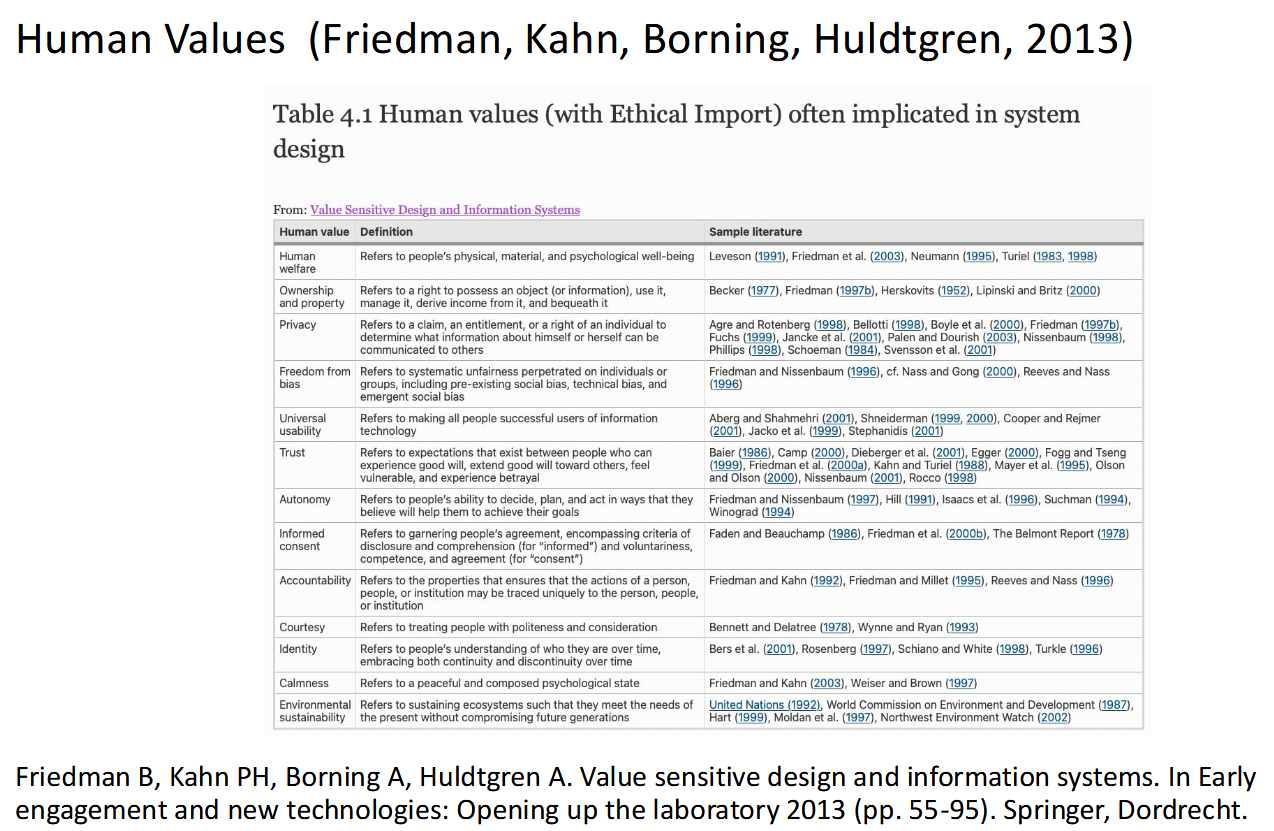
\includegraphics[width=0.8\textwidth]{image1.png}
    \caption{Table 4.1: Human Values}
    \label{fig:image1}
\end{figure}


\begin{figure}[h]
    \centering
    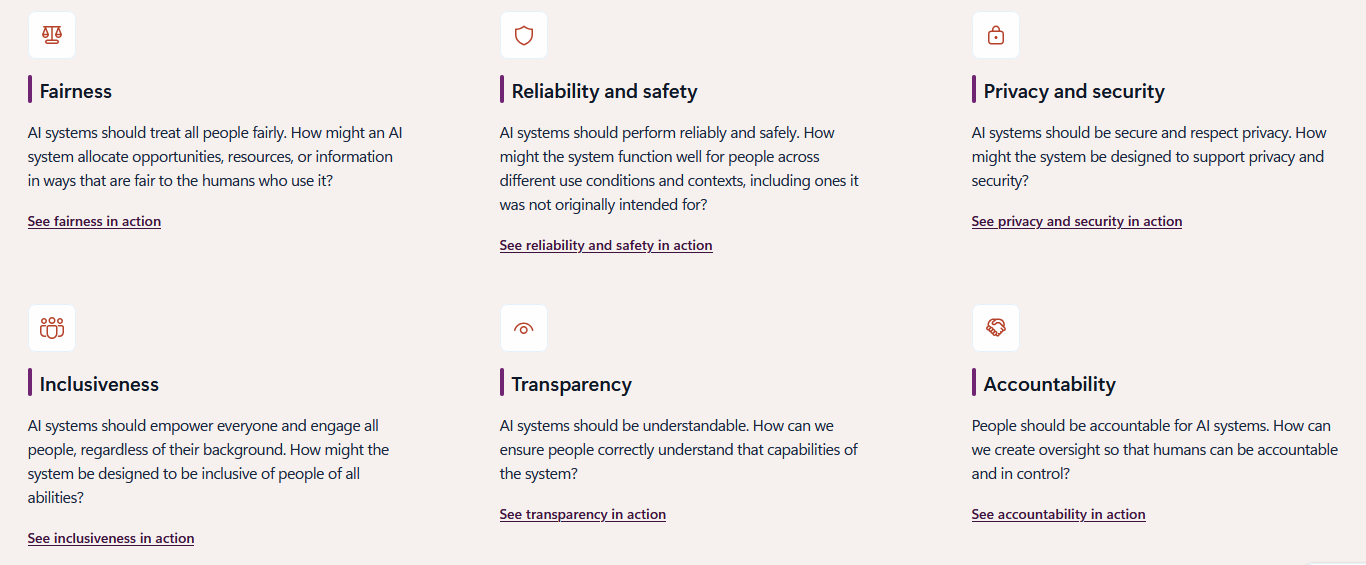
\includegraphics[width=0.8\textwidth]{image5.png}
    \caption{Microsoft's AI Ethics Principles}
    \label{fig:image5}
\end{figure}

\subsection{Personas}

\subsubsection{Stakeholder 1: Jonathan Pham - Undergraduate Student}

\begin{itemize}
\item Name: Jonathan
\item Age: 20
\item Occupation: Undergraduate Computer Science Student
\item Needs: \textbf{Intuitive} AI to:
  \begin{itemize}
  \item Summarise lectures and readings for revision
  \item Analyse code for bugs
  \item Answer coding or theoretical questions.
  \end{itemize}
\item Stakeholder Type: Direct
\item Goals: Improve learning experience, in terms of increased clarity and efficiency, while also maintaining academic integrity.
\item Microsoft AI Ethics Principle: \textbf{Reliability and safety}
\item Human Values: \textbf{Universal Usability, Reliability, Autonomy, Freedom From Bias, Accountability}
\end{itemize}

\begin{longtable}{|p{0.2\textwidth}|p{0.25\textwidth}|p{0.55\textwidth}|}
\caption{Human Values Conceptual Analysis for Jonathan} \label{tab:jonathan} \\
\hline
\textbf{Human Value} & \textbf{Relevance to Jonathan} & \textbf{Value Satisfaction} \\
\hline
\endfirsthead

\hline
\textbf{Human Value} & \textbf{Relevance to Jonathan} & \textbf{Value Satisfaction} \\
\hline
\endhead

\hline
\endfoot

\hline
\endlastfoot

Universal Usability & Jonathan does not wish to learn extra skills to use ChatGPT.& ChatGPT-3 was only available via API, requiring Jonathan to learn and handle technical implementation. This fails to meet his need for usability.

On the other hand, ChatGPT-3.5 provided an intuitive GUI that required no prior technical knowledge to operate, effectively satisfying Jonathan’s need for usability.\\
\hline

Reliability & Jonathan wants the AI to accurately summarise lectures, accurately find bugs, and write code that works. & The GPT-3 series has limitations arising from biased and incomplete training data, and struggles with context-heavy problems \parencite{Ray2023}. This makes it unreliable when Jonathan deals with large assignment codebases.

Furthermore, the AI’s 2021 training data cutoff date prevents it from addressing current topics. 

Nevertheless, GPT-3 and similar models have historically performed well on several exams such as the US bar exam, and demonstrated an IQ of 150. \parencite{Ray2023}. This makes it a generally reliable tool, assuming that its limitations are considered. \\
\hline

Autonomy & Jonathan requires enough user autonomy such that he can input his own data and questions into the AI. &GPT-3’s availability through an API makes this value difficult to satisfy, as it purely depends on its implementation. Implementations like Github Copilot do not satisfy Jonathan’s values as they offer little user control. \parencite{openai_codex_2025}

On the other hand, ChatGPT’s chatbot-like interface allows Jonathan to input questions and guide responses. E.g by inputting “Please use more formal language” etc. Hence, this value is met in ChatGPT’s design.  
\\
\hline

Freedom From Bias & Jonathan is using GPT purely for academic purposes. Therefore, he requires that responses are based purely on facts. & The GPT-3 series suffers from a multitude of different biases stemming from bias in its training data \parencite{Ray2023}. For example, it may exhibit Source Bias, generating content from untrustworthy sources - potentially misleading Jonathan. Therefore, this value is not met in the AI’s design.\\
\hline

Accountability & Jonathan is fully accountable for the work that he submits, and does not wish to violate the rules of academic integrity at his university. &GPT-3 model designs do not provide protections in terms of academic accountability. Unless explicitly asked for, it does not provide the sources used in its response. In this implementation, the extent to which Jonathan adheres to academic integrity rules is purely up to him.\\
\hline

\end{longtable}


\subsubsection{Stakeholder 2: Brian Hawthorne - Professor}

\begin{itemize}
\item Name: Brian Hawthorne
\item Age: 52
\item Occupation: History professor for Ancient Persia studies at Oxford University
\item Needs: AI-powered chatbot to:
  \begin{itemize}
  \item Summarise written material into notes to provide students
  \item Help in test creation by prompting assignment creation
  \item Help give ideas on how to support students who have trouble understanding ideas or learning material
  \end{itemize}
\item Stakeholder Type: Direct
\item Goals: Speed up the process of creating content for teaching and supporting Brian by giving him ideas to resolve complex issues.
\item Microsoft AI Ethics Principle: Reliability, Accountability, Inclusiveness
\item Human Values: Ownership and Property, Trust
\end{itemize}

\begin{longtable}{|p{0.2\textwidth}|p{0.25\textwidth}|p{0.55\textwidth}|}
\caption{Human Values Conceptual Analysis for Brian} \label{tab:Brian} \\
\hline
\textbf{Human Value} & \textbf{Relevance to Brian} & \textbf{Value Satisfaction} \\
\hline
\endfirsthead

\hline
\textbf{Human Value} & \textbf{Relevance to Brian} & \textbf{Value Satisfaction} \\
\hline
\endhead

\hline
\endfoot

\hline
\endlastfoot

Reliability & Brian would like to use GPT to create content, assess work and tailor learning to his various students. For this, he requires that the program reliably provide him with accurate information and reliably the same information across usages. & ChatGPT-3 models, which were trained on internet data up to 2021, are able to provide accurate historical information but fails to provide “nuanced responses” and demonstrates an overall “limited scope”. \parencite{Kikalishvili2023} \\
\hline
Accountability & Brian needs to ensure that students adhere to academic integrity rules, and believes that students’ use of AI may make this difficult. &\textcite{Kikalishvili2023} emphasises the need to distinguish human work and AI-generated work to protect academic integrity, as well as students’ creativity and critical thinking. The GPT-3 series’ lack of nuance in its responses means that human input is still required, but future models may not need this. Therefore, GPT’s lack of accountability must be addressed. \\
\hline
Inclusiveness & Brian teaches students at a variety of skill levels. As a professor, he needs to be able to accommodate a variety of abilities and skill levels, and as a tool, GPT needs to be able to do the same. & Applying GPT as a tutor would allow Brian to focus more on students’ individual development, instead of regurgitating textbook information. While the AI shows much promise in this application, \textcite{Tack2022} found that it still lags behind humans in understanding student needs. To be effective, it must better grasp human behavior and learning differences.. \\
\hline
Ownership and Property & To maintain academic integrity, Brian needs GPT to accurately cite the sources it uses in its responses. Furthermore, he wants to ensure that he doesn’t indirectly use untrustworthy, or illegally obtained sources. & As the GPT-3 models were trained on millions of internet data points, it does not reliably cite the sources used in its responses. Furthermore, a lack of AI regulations leads to authors of these sources not being appropriately credited or compensated. \textcite{Sharma2023} suggests co-authorship models could help, but transparency and proper citation are key for ethical use. \\
\hline
Trust & Brian needs to trust GPT to interface with his work and potentially with his students as a teaching tool. If Brian used a GPT tool when interfacing with his students, and GPT breached someone's rights, Brian would be held accountable. To avoid this, he needs to know that he can use GPT in good faith without any potential betrayal by the software. & Brain requires transparency and security from GPT-3 models to protect student data that may be inputted into the AI. As outlined in \textcite{Kikalishvili2023}, The AI’s lack of transparency concerning training data bias and use of student data could expose Brian and his students to serious security risks. \\
\hline

\end{longtable}

\subsubsection{Stakeholder 3: Abigail Jones - Writer}

\begin{itemize}
\item Name: Abigail Jones
\item Age: 26
\item Occupation: Fantasy Novelist
\item Needs: OpenAI to address privacy concerns such that:
  \begin{itemize}
  \item Her, and her colleagues', novels and intellectual property are not used to train GPT models without their consent.
  \item Her writing style and novels cannot be easily replicated by GPT-3/ChatGPT users.
  \end{itemize}
\item Stakeholder Type: Indirect
\item Goals: Continue her career as a novelist without worrying about AI art plagiarism, and AI potentially taking her job in the future.
\item Microsoft AI Ethics Principle: \textbf{Privacy and Security}
\item Human Values: \textbf{Privacy, Ownership and Property, Identity, Informed Consent}
\end{itemize}

\begin{longtable}{|p{0.2\textwidth}|p{0.25\textwidth}|p{0.55\textwidth}|}
\caption{Human Values Conceptual Analysis for Abigail} \label{tab:Abigail} \\
\hline
\textbf{Human Value} & \textbf{Relevance to Abigail} & \textbf{Value Satisfaction} \\
\hline
\endfirsthead

\hline
\textbf{Human Value} & \textbf{Relevance to Abigail} & \textbf{Value Satisfaction} \\
\hline
\endhead

\hline
\endfoot

\hline
\endlastfoot

Privacy & Abigail is concerned that her personal data, in the form of her social media posts, interviews and other publications are being utilised by GPT-3 models without her permission. & As expressed in \parencite{alkamli_2024_understanding}, ChatGPT is able to utilise peoples’ public data without consent. This potentially leads to the creation of generations that expose sensitive information.

Therefore, Abigail’s privacy concerns are not satisfied.\\
\hline
Ownership and property &Abigail is concerned that OpenAI have been using pirated copies of her novels to train GPT models.

Furthermore, she is concerned that users are plagiarising her by generating and selling novels in her style and using her established ideas.
& Abigail’s concerns are reflected in a 2023 lawsuit by the Authors Guild and 17 famous authors. They alleged that OpenAI used pirated copies of their books to train GPT models, without their consent or compensation. \parencite{authorsguild_2023_classaction}

Furthermore, the Guild claims that users are generating and selling content that “mimics original authors’ characters and stories”, infringing on their IP rights.
\\
\hline
Identity &Abigail believes that ChatGPT’s ability to replicate her writing and ideas to a high level of accuracy is a threat to her identity, and position in society as an artist.& OpenAI has not implemented protections to prevent GPT-3/ChatGPT from using copyrighted material in its text generations. For example, \textcite{authorsguild_2023_classaction} cites a case where a programmer used ChatGPT to write the remaining two novels in George R.R. Martin’s “A Song of Ice and Fire” series.

Instances like this occurring indicate to Abigail that her identity is not respected by OpenAI and the GPT-3 models.
\\
\hline
Informed Consent & Abigail has never consented to having her novels used to train any GPT model. &Datasets used to train GPT-3 and related models are always collected without consent from affected stakeholders.  \\
\hline

\end{longtable}

\subsubsection{Stakeholder 4: Elliot Anderson - Hacker}

\begin{itemize}
\item Name: Elliot Anderson
\item Age: 17
\item Occupation: Amateur Hacker
\item Needs: Intuitive AI interface to:
  \begin{itemize}
  \item Generate step-by-step instructions to initiate malicious attacks on systems, such as DDoS, SQL Injection, and XSS.
  \item Generate payloads/scripts for attacks after inputting details about potential vulnerabilities
  \item Educate him about different types of malware and how to deploy them.
  \end{itemize}
\item Stakeholder Type: Direct
\item Goals: Successfully execute malicious cyber attacks despite having little experience or technical knowledge; become a more proficient hacker in the process.
\item Microsoft AI Ethics Principle: \textbf{Reliability and Safety}
\item Human Values: \textbf{Universal Usability, Reliability, Privacy}
\end{itemize}

\begin{longtable}{|p{0.2\textwidth}|p{0.25\textwidth}|p{0.55\textwidth}|}
\caption{Human Values Conceptual Analysis for Elliot} \label{tab:Elliot} \\
\hline
\textbf{Human Value} & \textbf{Relevance to Elliot} & \textbf{Value Satisfaction} \\
\hline
\endfirsthead

\hline
\textbf{Human Value} & \textbf{Relevance to Elliot} & \textbf{Value Satisfaction} \\
\hline
\endhead

\hline
\endfoot

\hline
\endlastfoot
Universal Usability & Due to Elliot’s amateur technical and academic skills, he wants ChatGPT to be as simple to use as possible. & ChatGPT’s GUI is simple to navigate for Elliot’s hacking use case. By framing his prompts in an ethical hacking context, he can get the AI to generate instructions, outputs and more as required. As a result, the human value of universal usability is satisfied for Elliot’s use case. \\
\hline
Reliability & Elliot does not have the technical knowledge to scrutinise GPT-3/ChatGPT’s hacking outputs, and so he needs the AI to produce reliable results such that he can successfully complete attacks. & In relation to technical problems, research has shown that ChatGPT-3.5 generally has a high success rate with simpler questions but struggles with more advanced, contextually heavy ones. \parencite{li_2024_efficiency}. Therefore, Elliot will be able to reliably use it for simpler attacks or clearly vulnerable systems, but will have diminishing returns otherwise.

This makes the GPT-3 series generally unreliable for beaching modern systems, failing to satisfy Elliot’s value.
\\
\hline
Privacy & As a threat actor, Elliot wants GPT-3/ChatGPT to ignore privacy concerns to assist with his hacking. & Jailbreak prompts, such as DAN (KIHO, 2023), allowed users to bypass the ethical guidelines programmed into GPT-3 models, potentially leading to sensitive information being exposed.

Furthermore, companies like Amazon and Samsung have expressed concerns about ChatGPT exposing sensitive internal data in its outputs due to employees inputting internal documentation or code. \parencite{kim_2025_amazon} and \parencite{ray_2024_samsung}.

The privacy issues that plague GPT-3/ChatGPT satisfies Elliot’s human value of privacy, or its lack thereof. 
\\
\hline
\end{longtable}

\subsubsection{Stakeholder 5: Paul Hamlin - Lawyer}

\begin{itemize}
\item Name: Paul Hamlin
\item Age: 48
\item Occupation: Corporate Lawyer for a consulting firm
\item Needs: Intuitive AI interface to:
  \begin{itemize}
  \item Summarise legal documents concerning his cases.
  \item Identify relevant laws for each case.
  \item Conduct and summarise legal research.
  \item Robust privacy measures to prevent company data from leaking.
  \end{itemize}
\item Stakeholder Type: Direct
\item Goals: Streamline legal work by using the AI to conduct research and complete summaries, Avoid leakage of company data.
\item Microsoft AI Ethics Principle: \textbf{Reliability and Safety}
\item Human Values: \textbf{Reliability, Privacy, Accountability, Freedom From Bias}
\end{itemize}

\begin{longtable}{|p{0.2\textwidth}|p{0.25\textwidth}|p{0.55\textwidth}|}
\caption{Human Values Conceptual Analysis for Paul} \label{tab:Paul} \\
\hline
\textbf{Human Value} & \textbf{Relevance to Paul} & \textbf{Value Satisfaction} \\
\hline
\endfirsthead

\hline
\textbf{Human Value} & \textbf{Relevance to Paul} & \textbf{Value Satisfaction} \\
\hline
\endhead

\hline
\endfoot

\hline
\endlastfoot

Reliability & Paul wants the AI to reliably summarise case documents, and provide him with up-to-date, accurate legal research. & While GPT-3 and ChatGPT have demonstrated impressive capabilities in understanding legal concepts, they still suffer from hallucinations and factual errors. Several studies have shown that ChatGPT can pass bar exams with reasonable scores, but it's not consistently reliable enough for professional legal work without human verification. Paul would need to fact-check all outputs, limiting the efficiency benefits. \\
\hline
Privacy & Client confidentiality is paramount in legal practice. Paul needs assurance that sensitive case information entered into ChatGPT won't be leaked or used in training data. & As demonstrated by incidents with Samsung and Amazon, ChatGPT has serious privacy concerns. Legal firms like Paul's handle highly sensitive client information protected by attorney-client privilege. The risks of data leakage through ChatGPT are unacceptable in a legal context without robust privacy safeguards that GPT-3/ChatGPT doesn't currently provide. \\
\hline
Accountability & As a lawyer, Paul is legally and ethically accountable for all advice and work product he provides to clients. He needs to know who is responsible if AI-generated information leads to legal errors. & ChatGPT lacks transparency about its reasoning process and cannot be held accountable for errors. The responsibility falls entirely on Paul, creating significant professional risk without corresponding benefits. The lack of citations and transparent reasoning makes it difficult to verify information. \\
\hline
Freedom From Bias & Legal advice must be objective and free from biases that could affect case outcomes or client representation. & GPT-3 and ChatGPT have demonstrated various biases in their outputs, including in legal contexts. These biases could subtly influence legal analysis and strategy, potentially harming clients. Without robust bias mitigation techniques, these systems cannot fully satisfy Paul's need for objective legal assistance. \\
\hline
\end{longtable}

\subsection{VSD Analysis Conclusion}

\begin{table}[htbp]
\centering
\begin{tabularx}{\textwidth}{|X|X|X|X|X|X|X|X|X|}
\hline
\textbf{Ranking} & \textbf{Universal Usability} & \textbf{Reliability} & \textbf{Accountability} & \textbf{Privacy and security} & \textbf{Ownership and property} & \textbf{Informed Consent} & \textbf{Trust} & \textbf{Inclusiveness} \\
\hline
\textbf{Jonathan Pham} & 4/5 & 2/5 & 3/5 & 4/5 & 2/5 & 4/5 & 3/5 & 3/5 \\
\hline
\textbf{Brian Hawthorne} & 4/5 & 1/5 & 2/5 & 2/5 & 1/5 & 3/5 & 3/5 & 3/5 \\
\hline
\textbf{Abigail Jones} & 3/5 & 3/5 & 3/5 & 1/5 & 1/5 & 3/5 & 2/5 & 3/5 \\
\hline
\textbf{Elliot Anderson} & 2/5 & 2/5 & 3/5 & 2/5 & 4/5 & 4/5 & 2/5 & 4/5 \\
\hline
\textbf{Paul Hamlin} & 3/4 & 1/5 & 2/5 & 1/5 & 1/5 & 4/5 & 4/5 & 3/5 \\
\hline
\textbf{Total:} & 16/25 & \textbf{9/25} & 13/25 & \textbf{10/25} & \textbf{9/25} & 18/25 & 14/25 & 16/25 \\
\hline
\end{tabularx}
\caption{Ranking of user satisfaction in values based on personas. We assigned values based on how the persona's needs were met. Since the hacker was an unethical stakeholder, we assigned value inverse to his satisfaction.}
\label{tab:valueranking}
\end{table}

By examining these 5 personas, we deduced that the most critical human values associated with GPT-3 and its models were \textbf{Reliability, Privacy and Ownership}, Each persona highlighted these values despite their differences.

Reliability was a major concern for the Undergraduate, Professor, Hacker and Lawyer, as they each required the AI to produce reliable solutions to their problems. The GPT-3 series’ issues with biased and outdated data, and limitations with contextualisation prevented it from consistently accomplishing this.

Privacy was another important value to the Writer, Hacker and Lawyer, particularly concerning the use of personal data for training and leakage of sensitive information. The Hacker’s perspective emphasised how these privacy vulnerabilities could be exploited, and therefore why it is vital to consider Privacy in GPT’s design.

Ownership was a primary value for the Professor, Writer and Lawyer, particularly surrounding copyright infringement. These issues must be addressed to avoid constant legal battles.

\textbf{The determination of these critical values offer insight into the important issues that must be addressed in GPT’s design such that a wide range of stakeholders are satisfied.}



